%-----------------------------CAPITOLO 2
\section{Large Hadron Collider (LHC)}
    Il Large Hadron Collider (LHC) è l’acceleratore di particelle più grande al mondo ed è situato al laboratorio CERN (Organizzazione Europea per la Ricerca Nucleare) presso Ginevra in Svizzera. Questo imponente strumento scientifico rappresenta il vertice della ricerca nel campo della fisica delle particelle ed è progettato con l’obiettivo di sondare i segreti più profondi dell’universo e comprendere le leggi fondamentali della natura.
    
    L’acceleratore è costituito da un anello circolare di circa \qty{27}{\kilo \meter} di circonferenza, situato in un tunnel a circa \qty{100}{\meter} sotto terra, all’interno del quale vengono fatti circolare fasci di particelle a velocità prossime a quella della luce. Prima di essere immesse in LHC le particelle vengono accelerate da un complesso sistema di pre-acceleratori, vedi figura~\ref{fig:2-1-CERN-accelerator-complex}, che ne incrementano in passi successivi l’energia cinetica fino a poter essere iniettate dentro l’anello di LHC e portate all’energia di collisione. In LHC potenti magneti superconduttori mantengono i fasci in un moto circolare e cavità a radiofrequenza forniscono il campo elettrico che incrementa l’energia delle particelle ad ogni passaggio. I magneti sono mantenuti nello stato di superconduttività grazie ad un sistema di raffreddamento a elio liquido che mantiene gli speciali cavi elettrici che compongono le bobine ad una temperatura di \qty{-271}{\degreeCelsius}.
    
    Raggiunte le energie di design dell'acceleratore, i fasci vengono fatti collidere in punti specifici dove si trovano gli esperimenti: i quattro principali rivelatori di LHC sono chiamati ATLAS, CMS, LHCb e ALICE.

    \textbf{ATLAS} e \textbf{CMS} sono i rivelatori più grandi e sono general-purpose, ovvero non hanno un unico obbiettivo specifico di ricerca, bensì esplorano vari aspetti della fisica delle particelle. Essi lavorano in maniera indipendente l’uno dall’altro nonostante facciano ricerca sugli stessi aspetti della fisica. Il motivo di questa ``competizione'' è quello di effettuare le stesse misure sperimentali facendo due ricerche separate per convalidare in maniera più efficace i risultati ottenuti. Ad esempio, ATLAS e CMS sono stati responsabili della scoperta del Bosone di Higgs nel 2012.

    ALICE e LHCb sono invece esperimenti specializzati in particolari fenomeni:
    \begin{description}
        \item[LHCb] si occupa di indagare le sottili differenze tra materia e antimateria attraverso lo studio dettagliato di adroni contenenti quark bottom $b$.

        \item[ALICE] si concentra sullo studio delle collisioni tra ioni pesanti, come spiegato nel capitolo~\ref{cha:1-QCD}, con la conseguente produzione di QGP, vedi la sezione~\ref{sec:QGP}, in sostanza nello studio delle fasi iniziali della vita dell’universo dopo il Big Bang.
    \end{description}

    \begin{figure}[h]
        \centering
        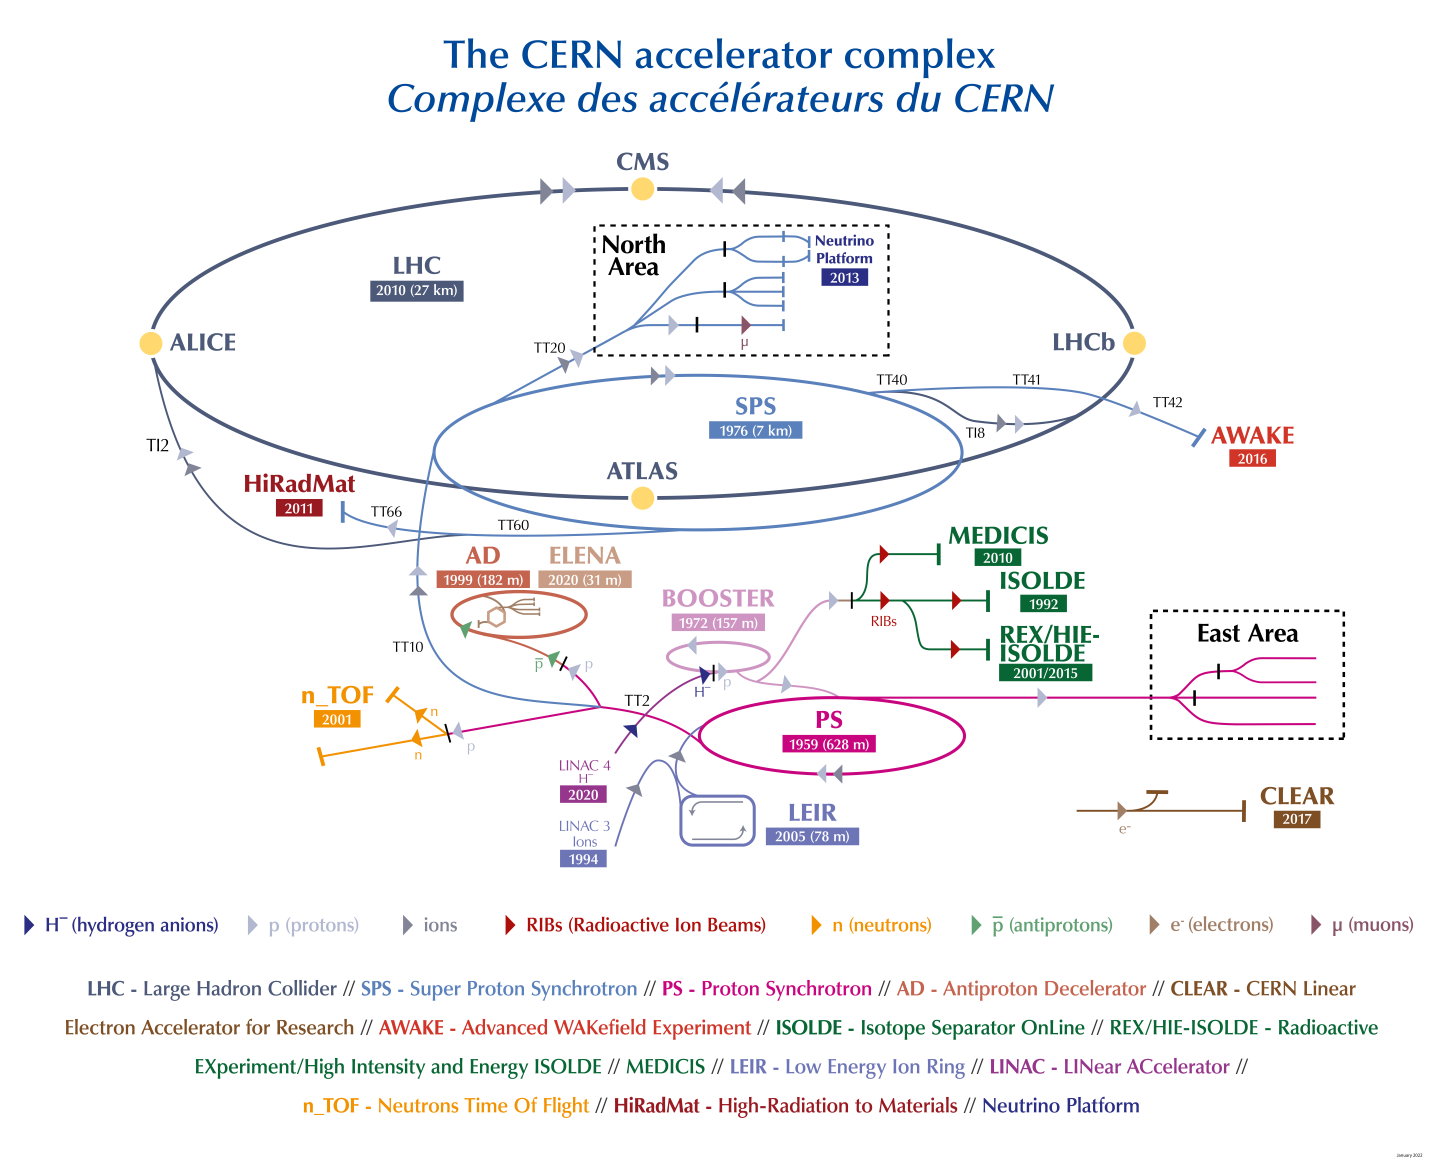
\includegraphics[width=0.8\linewidth]{res/fig/2-chapter/1-CERN-accelerator-complex.png}
        \caption{Sistema di rivelatori e acceleratori degli esperimenti del CERN di Ginevra~\cite{Lopienska_2022}.}
        \label{fig:2-1-CERN-accelerator-complex}
    \end{figure}


\section{A Large Ion Collider Experiment (ALICE)}
    ALICE: A Large Ion Collider Experiment~\cite{ALICE_2008} è un \textit{rivelatore} progettato per studiare principalmente la QCD, vedi sezione~\ref{sec:QCD}, e più in generale la materia nucleare in condizioni estreme di temperatura e di densità di energia. Il rivelatore è stato costruito da una collaborazione che comprende più di 1000 fisici e ingegneri da 30 paesi del mondo. Rappresentato in figura~\ref{fig:2-2-ALICE-detector} ha una dimensione di \qtyproduct[product-units = bracket-power]{16 x 16 x 26}{\metre} e un peso complessivo di 10\,000 tonnellate.
    
    ALICE è composto da una parte centrale dedicata alla misura di adroni, elettroni e fotoni e da uno spettrometro a muoni che copre la regione ad alta rapidità. La parte centrale copre angoli polari da \ang{45} a \ang{135} ed è integrata in un grande magnete solenoidale riutilizzato dall’esperimento L3 che operava al precedente acceleratore, il Large Electron-Positron collider (LEP).
    
    L’esperimento è composto da 18 differenti sistemi o rivelatori, come mostrato in figura~\ref{fig:2-2-ALICE-detector}, ognuno con la propria tecnologia specifica, ottimizzato in base ai requisiti fisici e alle condizioni ambientali alle quali è previsto che operi. Il vincolo di progettazione più severo consiste nel riuscire a sopportare l’ingente molteplicità carica prevista per collisioni \ch{Pb}-\ch{Pb} centrali. I diversi rivelatori sono stati ottimizzati per fornire una elevata \textit{risoluzione} in impulso e un’eccellente \textit{identificazione} delle particelle su un ampio intervallo di quantità di moto, fino alle molteplicità più elevate previste per LHC. Ciò consente una completa analisi dei segnali di adroni, elettroni, muoni e fotoni prodotti nelle collisioni.

    \begin{figure}[t]
        \centering
        \includegraphics[width=1\linewidth]{res/fig/2-chapter/2-ALICE-detector.pdf}
        \caption{Spaccato del rivelatore ALICE con indicati i 18 sottorivelatori~\cite{Tauro_2017}.}
        \label{fig:2-2-ALICE-detector}
    \end{figure}
    
    Dall’interno verso l’esterno, la parte centrale contiene, vedi figura~\ref{fig:2-3-ALICE-detector-center}:
    \begin{enumerate}
        \item Inner Tracking System (ITS) composto da sei piani di rivelatori al silicio con elevata risoluzione spaziale,

        \item Camera a Proiezione Temporale (Time Projection Chamber TPC),
        
        \item rivelatori di Radiazione di Transizione (Transition Radiation Detector TRD),

        \item rivelatore per la misura del Tempo di Volo (Time Of Flight TOF) delle particelle cariche,

        \item rivelatore Cherenkov ad Immagini ad Anello (High Momentum Particle Identification HMPID) e due calorimetri elettromagnetici (PHOton Spectrometer PHOS e Electro Magnetic Calorimeter EMCal).
    \end{enumerate}
    Tutti i rivelatori, eccetto HMPID, PHOS e EMCal, coprono l’intero angolo azimutale~\cite{ALICE_2008}.

\newpage

    \begin{figure}[t]
        \centering
        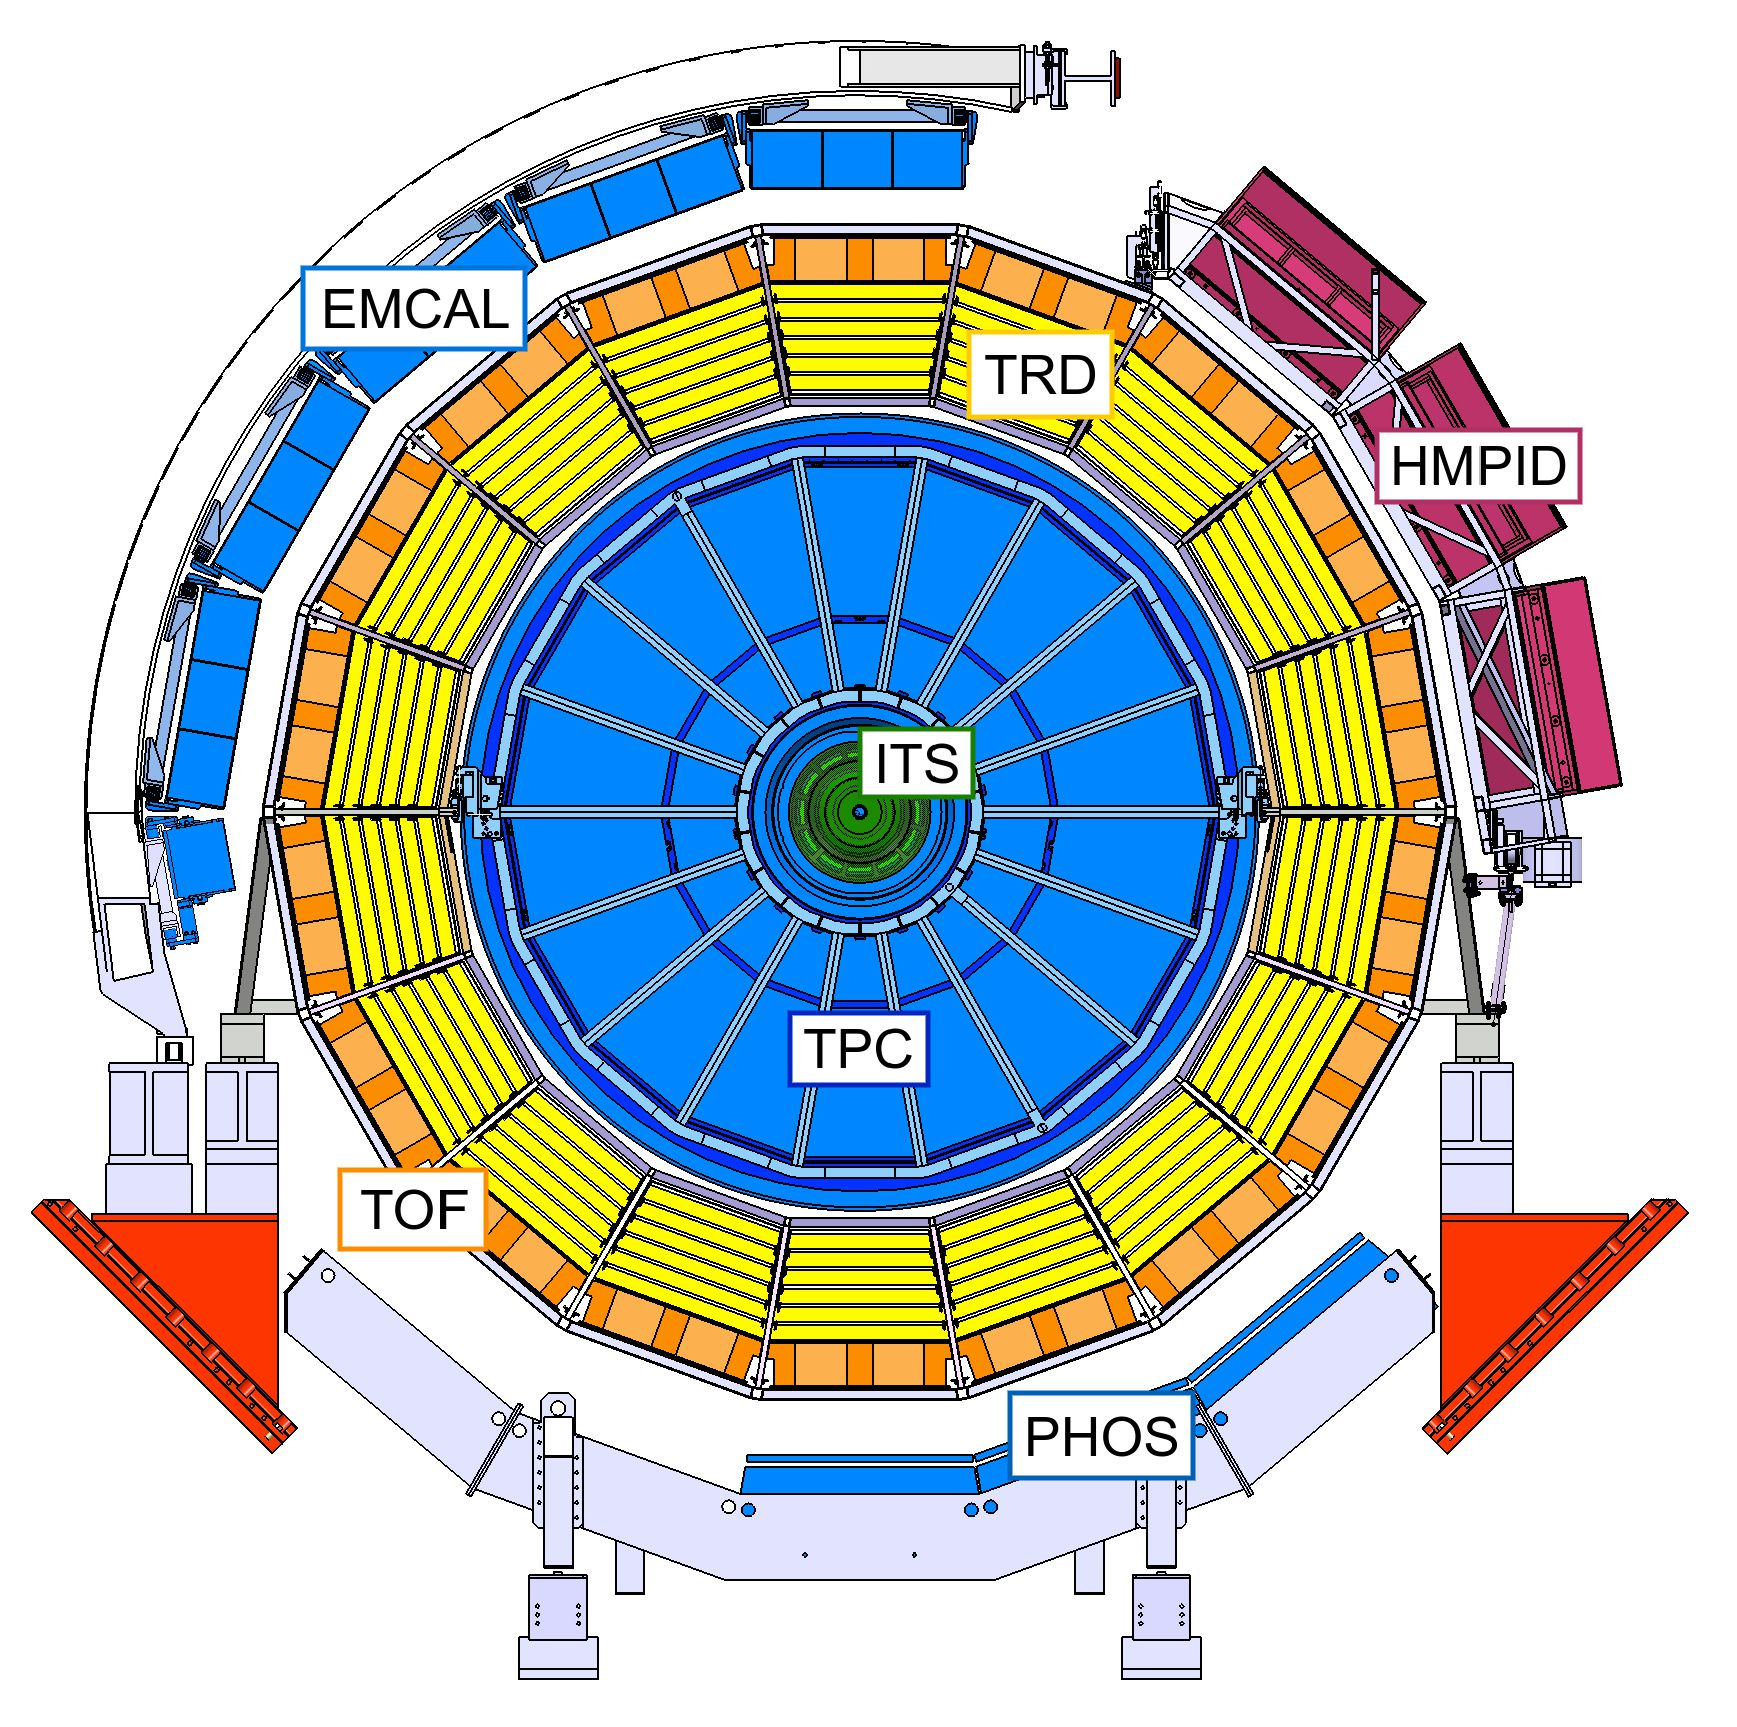
\includegraphics[width=0.6\linewidth]{res/fig/2-chapter/3-ALICE-detector-center.jpg}
        \caption{Sezione trasversale della parte centrale del rivelatore ALICE~\cite{Gagliardi_2019}.}
        \label{fig:2-3-ALICE-detector-center}
    \end{figure}

    \subsection{Considerazioni sulla costruzione}
        La costruzione e il design di ALICE sono stati guidati da specifici requisiti fisici e dalle condizioni sperimentali per le collisioni di particelle, originariamente pensate essere per eventi nucleo-nucleo, per poi svilupparsi anche in eventi protoni-protoni.

        ALICE è l’unico esperimento a LHC espressamente progettato per lo studio della materia nucleare creata in collisioni di ioni pesanti relativistici e del QGP. Per questo motivo esso dovrà coprire il maggior numero di osservabili possibili studiando tutti i diversi fenomeni riconducibili alla formazione di uno stato di QGP insieme alle informazioni globali che possono descrivere l’evoluzione dinamica del sistema creato nel punto di collisione e la sua termodinamica. Le caratteristiche \textit{globali} dell’evento come la molteplicità carica delle interazioni e il flusso di energia trasversa o a zero gradi definiscono la \textit{geometria} della collisione: parametro di impatto, forma e orientamento della fireball, il volume di collisione, così come il \textit{numero} di nucleoni interagenti nell’urto. Lo studio della produzione di adroni contenenti quark pesanti (charm e bottom) e i processi di frammentazione dei jet permettono di esplorare la \textit{cinematica} dei partoni e la loro perdita di energia per interazione con il mezzo partonico ad alta densità. Il \textit{flusso ellittico} è un osservabile sensibile alle proprietà fluidodinamiche del QGP, come la viscosità. Lo studio dei \textit{fotoni diretti} può rivelare la formazione di un QGP in equilibrio termico. La produzione soppressa o aumentata di \textit{stati di quarkonia} può essere utilizzata per studiare il deconfinamento e la ricombinazione partonica, mentre lo studio delle \textit{risonanze} permette di investigare il ripristino della simmetria chirale e, insieme ai \textit{rapporti di produzione} tra diverse specie di particelle, agli spettri e alle distribuzioni in impulso trasverso, l’\textit{evoluzione dinamica} del sistema da una fase deconfinata a quella adronica.

        La progettazione dell’esperimento ALICE è stata guidata dai requisiti fisici oltre che dalle condizioni sperimentali attese nelle collisioni nucleo-nucleo a LHC. ALICE è stato progettato per operare a \textit{molteplicità} fino a 8000 particelle cariche per unità di rapidità, estrapolando i valori misurati nei precedenti esperimenti con collisioni nucleo-nucleo ad energie inferiori. Questa alta molteplicità, unita a \textit{luminosità} attese in collisioni Pb-Pb a LHC moderate, ha portato alla scelta di \textit{rivelatori lenti ma ad elevata granularità} (come la TPC e le camere SSD), immersi in un debole campo magnetico solenoidale da \qty{0.5}{\tesla}.

        Un \textit{preciso tracciamento}, insieme ad una elevata risoluzione in impulso e capacità di identificazione delle diverse particelle prodotte durante l’evoluzione del sistema sono caratteristiche distintive dell’esperimento ALICE. La misura dell’impulso delle particelle prodotte deve poter essere effettuata su un largo intervallo che si estende per oltre tre ordini di grandezza, dalle decine di \unit[per-mode = symbol]{\mega \eV \per \clight} per lo studio di effetti collettivi fino a ben oltre \qty[per-mode = symbol]{100}{\giga \eV \per \clight} per la fisica dei jet. Ciò si ottiene con una combinazione di material budget molto basso per ridurre il multiple scattering a basso impulso trasverso $p_{T}$ (13\% X0 fino all’estremità esterna della TPC) e un ampio braccio di leva di tracciamento fino a \qty{3.5}{\meter} per garantire una buona risoluzione ad alto impulso $p_{T}$.

    \subsection{Particle Identification (PID)}
        ALICE si concentra sulla fisica a rapidità\footnote{La \textit{rapidità} è una grandezza adimensionale che è basata sul rapporto tra l’energia e la componente del momento lungo l’asse della collisione di una particella. È una misura alternativa dell’energia cinetica di una particella utilizzata frequentemente nelle collisioni ad alta energia perché ha proprietà utili sotto trasformazioni di Lorentz.} centrali $\abs{\eta} <$ \num{1} come ad esempio la regione a più bassa concentrazione barionica e massima densità energetica. L’identificazione di particelle (Particle Identification, PID) su tutto il range di momenti $p_{T}$ è essenziale siccome molti altri osservabili sono dipendenti o dalla massa o dal sapore della particella.

        In ALICE vengono utilizzate quasi tutte le tecniche di PID note: perdita specifica di energia di ionizzazione $\dd{E}/\dd{x}$, time of flight (sezione~\ref{sec:2-TOF}), radiazione di transizione e radiazione Cherenkov, calorimetria elettromagnetica, rivelatori di muoni e ricostruzione topologica dei decadimenti.

        Nonostante tutte queste tecniche di identificazione, è molto difficile selezionare segnali di decadimenti di sapori pesanti, come nel nostro caso quello della $\Lambda_{c}^{+}$, vedi capitolo~\ref{cha:3-LAMBDA+c}: è dunque richiesta l’acquisizione di un’enorme quantità di eventi con un alta efficienza del sistema di Data Acquisition (fino ad una frequenza di \qty[per-mode = symbol]{1.3}{\giga \byte \per \second} su memoria fissa) per registrare un numero di eventi dell’ordine di grandezza di \num{E7} in sole poche settimane.
        
        Di seguito sono elencati i rivelatori di ALICE le cui informazioni sono state utilizzate nell’analisi presentata nel capitolo~\ref{cha:3-LAMBDA+c}.

\section{Inner Tracking System (ITS)}
    L’Inner Tracking System (ITS), schematizzato in figura~\ref{fig:2-4-ALICE-ITS} circonda la beam pipe (il tubo a vuoto all'interno del quale circolano i protoni e gli ioni) in cui scorre il fascio di particelle e consiste di sei strati cilindrici coassiali di rivelatori al silicio, localizzati da un raggio minimo di \qty{4}{\centi \meter}, imposto dalle dimensioni della beam pipe, a un raggio massimo di \qty{43}{\centi \meter}, necessario per il matching delle traiettorie con il successivo rilevatore, la TPC.
    
    ITS copre un intervallo di pseudorapidità di $\abs{\eta} <$ \num{0.9} e i suoi obiettivi sono:
    \begin{itemize}
        \item[-] la \textit{localizzazione} dei vertici primario e secondario,

        \item[-] il \textit{tracciamento} e l’\textit{identificazione} di particelle con momento inferiore a \qty[per-mode = symbol]{200}{\mega \eV \per \clight} e

        \item[-] il miglioramento della \textit{misura} del parametro d’impatto e dell’impulso delle differenti particelle cariche effettuata dalla TPC.
    \end{itemize}
    
    Per ottenere una risoluzione adeguatamente alta del parametro d’impatto, data l’elevata densità di particelle attesa nelle collisioni tra ioni pesanti a LHC (circa \num{50} particelle/\unit{\centi \meter^2}), sono stati scelti i Silicon Pixel Detectors (SPD) per i primi due strati a partire dall’interno e i Silicon Drift Detectors (SDD) per i successivi due. Per gli ultimi due strati, dove la densità di particelle prevista è ridotta a una particella/\unit{\centi \meter^2}, sono stati scelti i Silicon micro-Strip Detectors (SSD). I quattro strati più esterni hanno un readout analogo e possono essere usati per la Particle Identification attraverso la misura della perdita di energia $\dd{E}/\dd{x}$ nella regione non relativistica.

    \begin{figure}[h]
        \centering
        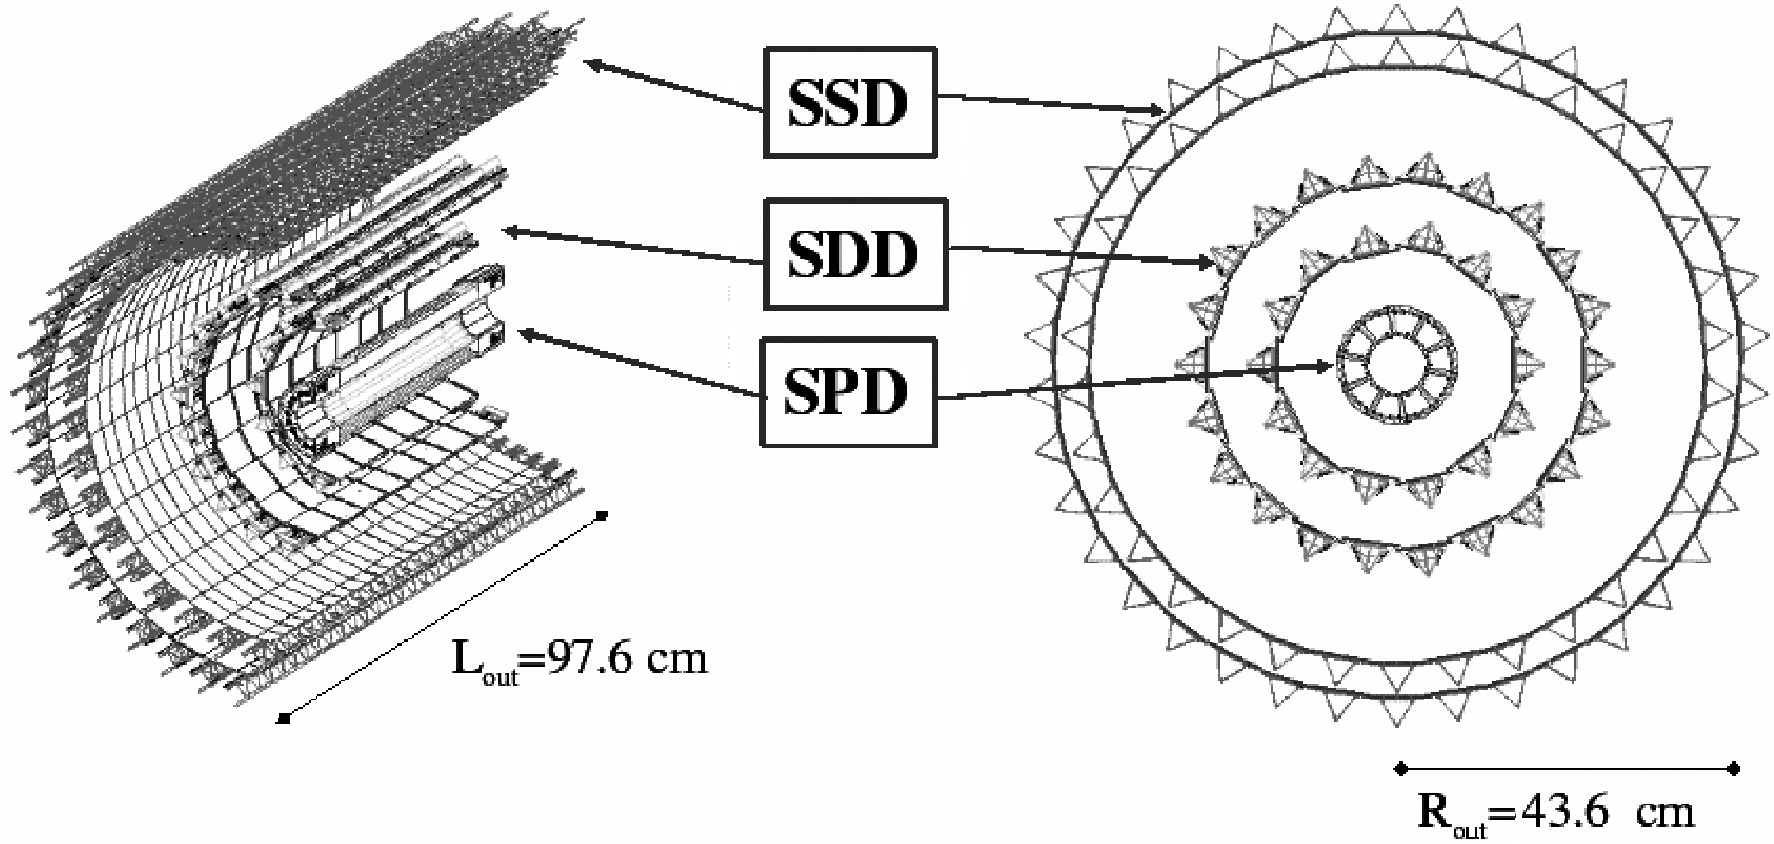
\includegraphics[width=1\linewidth]{res/fig/2-chapter/4-ALICE-ITS.jpg}
        \caption{Spaccato e sezione interna dell'ITS di ALICE~\cite{ALICE_2008}.}
        \label{fig:2-4-ALICE-ITS}
    \end{figure}

\section{Time Projection Chamber (TPC)}
    La Time-Projection Chamber (TPC), mostrata in figura~\ref{fig:2-5-ALICE-TPC}, è il principale rilevatore del central barrel per il \textit{tracciamento} delle particelle. I suoi scopi sono di fornire misure precise di \textit{impulso} delle particelle cariche in un range di $p_{T}$ di \qtyrange[per-mode = symbol, range-phrase = --, range-units = single]{0.1}{100}{\giga \eV \per \clight}, attuare l’\textit{identificazione} delle particelle e la \textit{localizzazione} dei vertici di decadimento. La TPC ha una simmetria cilindrica, coassiale con la direzione del fascio, con una zona attiva compresa tra un raggio interno di \qty{85}{\centi \meter} e uno esterno di \qty{250}{\centi \meter}.

    \begin{figure}[h]
        \centering
        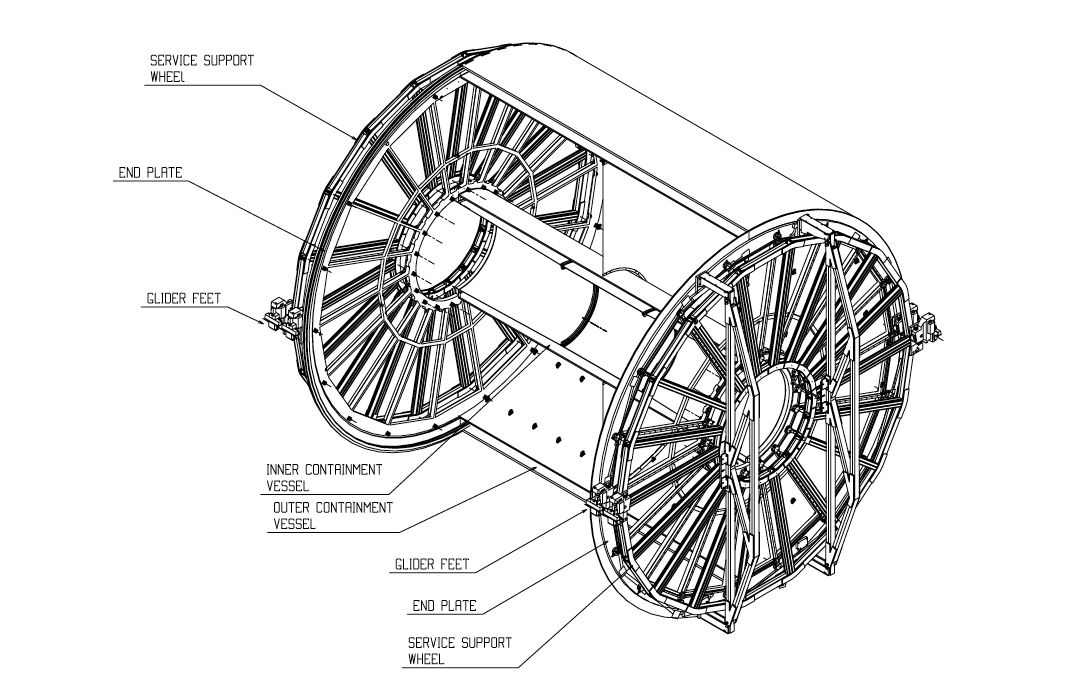
\includegraphics[width=0.76\linewidth]{res/fig/2-chapter/5-ALICE-TPC.jpg}
        \caption{Rappresentazione schematica della struttura della TPC di ALICE~\cite{Korcari_2017}.}
        \label{fig:2-5-ALICE-TPC}
    \end{figure}

    L’interno del rivelatore è riempito con \qty{90}{\meter^3} di una miscela di \ch{Ne}--\ch{CO2}--\ch{N2} in percentuali \qtylist{85;10;5}{\percent} rispettivamente. Quando questo gas è attraversato da una particella carica, viene ionizzato creando una traccia formata da elettroni liberi e lacune. Questi vengono guidati tramite un campo elettrico interno alle readout chambers, presenti sulle due basi del cilindro e composte da rivelatori Gas Electron Multipliers e composte da Multi-Wire Proportional Chambers (MWPCs), montate su 18 settori di forma trapezoidale).

\begin{comment}
    qui c'è una incongruenza di cui non mi ero accorto ai tempi della tesi di Giacomelli... stiamo descrivendo il primo rivelatore ALICE (con i 6 layer di silicio dell'ITA diviso in SPD, SDD e SSD). Quindi ai tempi la TPC aveva come readout chemaber delle MWPC. Quindi qui è più corretto scrivere
\end{comment}
    
    La posizione degli hit sulle camere di readout, in aggiunta alla posizione lungo l’asse $z$, determinata misurando il tempo di arrivo del segnale sugli endcap della TPC, permettono un tracciamento digitale in 3 dimensioni della traccia rilasciata dalla particella carica. Ricostruendo l’intera traiettoria e il suo raggio di curvatura è possibile risalire all’impulso della particella carica che l’ha generata.
    
    La PID viene effettuata attraverso la misura della ionizzazione specifica delle particelle $\dd{E}/\dd{x}$. Riportando questa misura in funzione dell’impulso della particella è possibile distinguere le diverse specie, come riportato in figura~\ref{fig:2-6-ALICE-pp13.6TeV-performance}. Questa tecnica permette un'ottima separazione nella regione $1/\beta^2$ della Bethe-Bloch e ad alti $p_{T}$ quando inizia la risalita relativistica. Per momenti intermedi invece è necessario utilizzare altre tecniche di identificazione come ad esempio quella del Time-Of-Flight (TOF), sezione~\ref{sec:2-TOF}.

%\clearpage

    \begin{figure}[p]
        \centering
        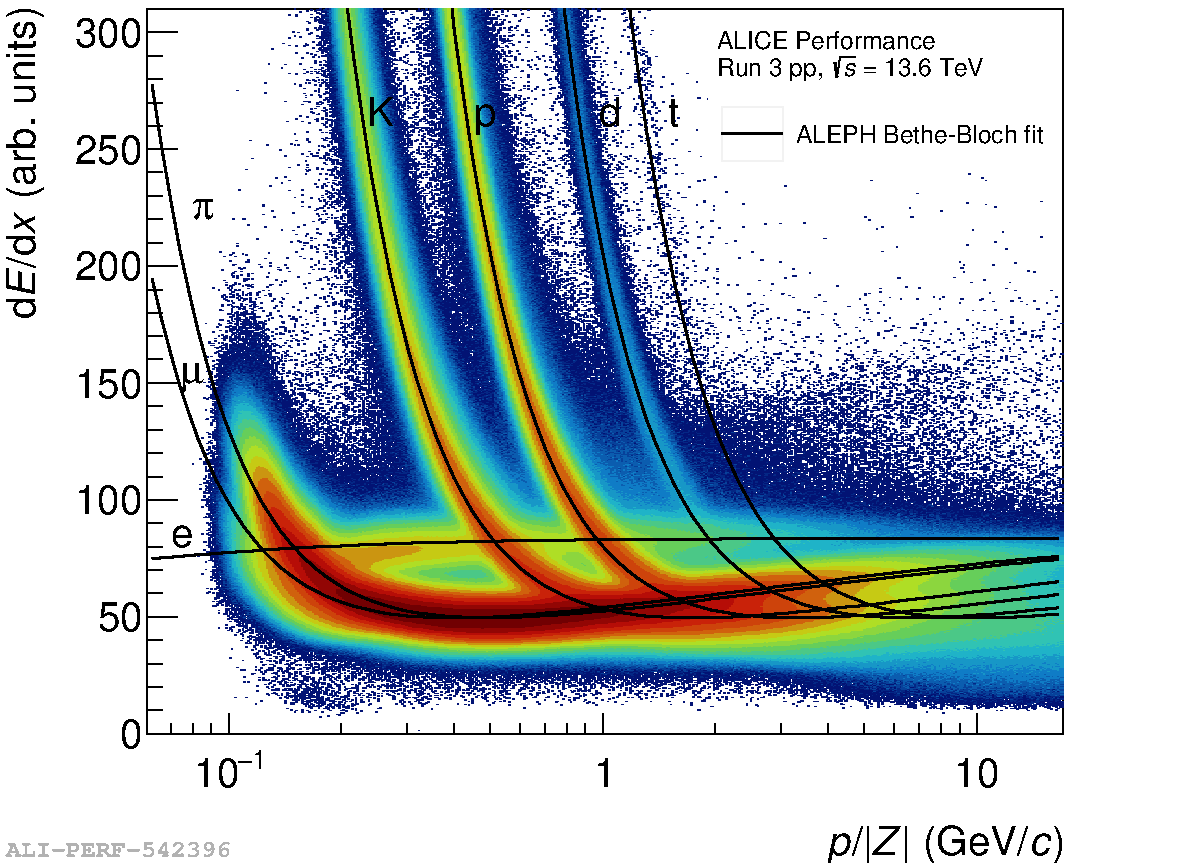
\includegraphics[width=1\linewidth]{res/fig/2-chapter/6-ALICE-pp13.6TeV-performance.pdf}
        \caption{Misura della ionizzazione specifica in funzione dell’impulso della particella, è possibile notare come l’andamento vari in base al tipo di particella osservata~\cite{ALICE-pp13.6TeV-performance}.}
        \label{fig:2-6-ALICE-pp13.6TeV-performance}
    \end{figure}

%\clearpage

\section{Time Of Flight (TOF)}
\label{sec:2-TOF}
    Il rilevatore Time-Of-Flight (TOF) di ALICE, mostrato in figura~\ref{fig:2-7-ALICE-TOF} ha un ruolo fondamentale nella Particle Identification nel range di \textit{impulsi intermedi}: è in grado di separare pioni e kaoni per $p_{T} <$ \qty[per-mode = symbol]{2.5}{\giga \eV \per \clight} e kaoni e protoni per $p_{T} <$ \qty[per-mode = symbol]{4}{\giga \eV \per \clight}, nell’intervallo di pseudorapidità $\abs{\eta} <$ \num{0.9}. Il TOF fornisce \textit{misure sul tempo di volo} di ciascuna particella carica; questa informazione, combinata con le misure della lunghezza della traiettoria percorsa e dell'impulso della particella carica fornite da ITS e TPC, permette di calcolare la massa di tale particella e quindi di determinarne l'identità, tramite la formula:
    \begin{equation}
        \beta = \frac{v}{c} = \frac{L}{tc} = \frac{1}{\sqrt{\left(\frac{mc}{p}\right)^2 +1}} \to m = \frac{p}{c} \sqrt{\frac{c^2t^2}{L^2} - 1}
    \end{equation}
    
    Come i rivelatori precedentemente mostrati, il TOF ha una forma cilindrica coassiale alla beam pipe ed è situato a una distanza di \qty{3.8}{\meter} da quest’ultima. È formato da 1638 Multi-gap Resistive Plate Chambers (MRPC) raggruppati in 18 settori azimutali, ciascuno a sua volta suddiviso in 5 moduli contenenti diversi MRPC in base alla posizione: 15 per i moduli centrali e 19 per quelli intermedi o esterni.

    \begin{figure}[h]
        \centering
        \includegraphics[width=0.62\linewidth]{res/fig/2-chapter/7-ALICE-TOF.eps}
        \caption{Rappresentazione schematica della struttura del TOF di ALICE~\cite{ALICE_TOF_2017}.}
        \label{fig:2-7-ALICE-TOF}
    \end{figure}

    Un esempio di Identificazione di Particelle con il rivelatore TOF è riportato in figura in cui la velocità delle particelle cariche è riportata in funzione del loro impulso.

    La figura~\ref{fig:2-8-ALICE-PbPb5.02TeV-performance} illustra come avviene l'identificazione delle particelle tramite il rivelatore TOF. Nel grafico è riportata la velocità delle particelle cariche, misurata dal rivelatore in collisioni Pb-Pb ad energie del centro di massa di \qty{5.02}{\tera \eV} per coppie di nucleoni, in funzione del loro impulso; le bande più popolate rappresentano le diverse specie. La differenza tra velocità misurata e velocità attesa per ogni ipotesi di massa della particella, divisa per la risoluzione temporale del rivelatore, costituisce il \textit{potere di separazione} del rivelatore.

    \begin{figure}[p]
        \centering
        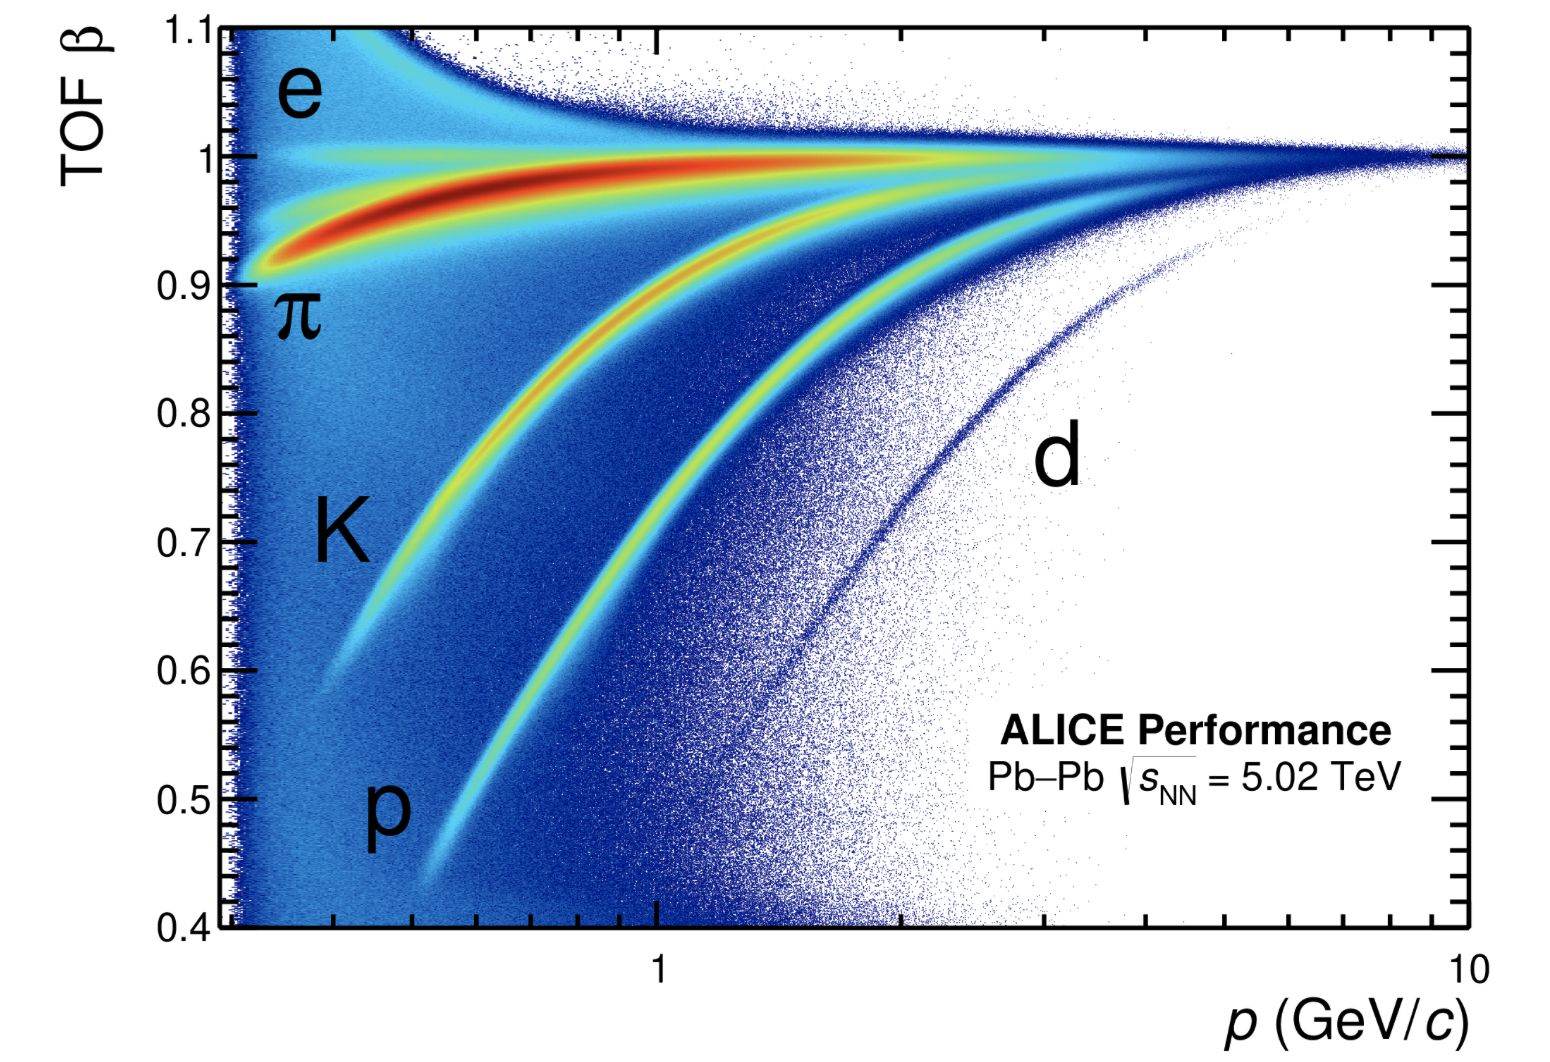
\includegraphics[width=1\linewidth]{res/fig/2-chapter/8-ALICE-PbPb5.02TeV-performance.jpg}
        \caption{Velocità delle particelle cariche in funzione del loro impulso~\cite{ALICE-PbPb5.02TeV-performance}.}
        \label{fig:2-8-ALICE-PbPb5.02TeV-performance}
    \end{figure}